\documentclass{beamer}
\usepackage[utf8]{inputenc}

\usetheme{Madrid}
\usecolortheme{default}
\usepackage{amsmath,amssymb,amsfonts,amsthm}
\usepackage{txfonts}
\usepackage{multicol}
\usepackage{tkz-euclide}
\usepackage{listings}
\usepackage{adjustbox}
\usepackage{array}
\usepackage{tabularx}
\usepackage{gvv}
\usepackage{lmodern}
\usepackage{circuitikz}
\usepackage{tikz}
\usepackage{graphicx}
\usepackage{hyperref}

\setbeamertemplate{page number in head/foot}[totalframenumber]

\usepackage{tcolorbox}
\tcbuselibrary{minted,breakable,xparse,skins}



\definecolor{bg}{gray}{0.95}
\DeclareTCBListing{mintedbox}{O{}m!O{}}{%
  breakable=true,
  listing engine=minted,
  listing only,
  minted language=#2,
  minted style=default,
  minted options={%
    linenos,
    gobble=0,
    breaklines=true,
    breakafter=,,
    fontsize=\small,
    numbersep=8pt,
    #1},
  boxsep=0pt,
  left skip=0pt,
  right skip=0pt,
  left=25pt,
  right=0pt,
  top=3pt,
  bottom=3pt,
  arc=5pt,
  leftrule=0pt,
  rightrule=0pt,
  bottomrule=2pt,
  toprule=2pt,
  colback=bg,
  colframe=orange!70,
  enhanced,
  overlay={%
    \begin{tcbclipinterior}
    \fill[orange!20!white] (frame.south west) rectangle ([xshift=20pt]frame.north west);
    \end{tcbclipinterior}},
  #3,
}
\lstset{
    language=C,
    basicstyle=\ttfamily\small,
    keywordstyle=\color{blue},
    stringstyle=\color{orange},
    commentstyle=\color{green!60!black},
    numbers=left,
    numberstyle=\tiny\color{gray},
    breaklines=true,
    showstringspaces=false,
}
%------------------------------------------------------------
%This block of code defines the information to appear in the
%Title page
\title %optional
{9.4.16}
\date{October 4,2025}
%\subtitle{A short story}

\author % (optional)
{Aditya Appana - EE25BTECH11004}



\begin{document}


\frame{\titlepage}
\begin{frame}{Question}
Find the roots of the following quadratic equation graphically:
$$2x^2-7x+3=0$$
\end{frame}



\begin{frame}[fragile]
    \frametitle{Solution}
The parabola can be represented in vector form as:
\begin{align}
    \vec{x^T}\myvec{1&0\\0&0}\vec{x} - \myvec{7/2 \\ 1/2}^T\vec{x} + \frac{3}{2} = 0
\end{align}\\
The y-axis can be represented in vector form as:
\begin{align}
    \vec{x} = \kappa\myvec{1\\0}
\end{align}\\
We need to find the intersection of this line with the parabola, which can be done by substituting equation (2) in (1):
\end{frame}


\begin{frame}[fragile]
    \frametitle{Solution}
\begin{align}
    \kappa\myvec{1\\0}^T\myvec{1&0\\0&0}\kappa\myvec{1\\0} - \myvec{7/2 \\ 1/2}^T\kappa\myvec{1\\0} + \frac{3}{2} = 0\\
    2\kappa^2-7\kappa+3=0\\
    (2\kappa - 1)(\kappa -  3) = 0\\
    \kappa = \frac{1}{2}, 3
\end{align}\\
Therefore, the points of intersection \textit{i.e.} the \textbf{roots} are $\myvec{0.5\\0}$ and $  \myvec{3\\0}$.
\end{frame}


\begin{frame}[fragile]
    \frametitle{Python Code}
    \begin{lstlisting}
import matplotlib.pyplot as plt
import numpy as np

x = np.linspace(-10,15,100)
y = 2*x*x - 7*x + 3
zero = np.zeros(100)

fig = plt.figure(figsize = (6,6))
ax = fig.add_subplot(111)

plt.plot(x,y, label='$2x^2 - 7x + 3$')
ax.scatter(3,0, label='(3,0)',color='green')
ax.scatter(0.5,0, label = '(0.5,0)', color = 'red')
plt.plot(x,zero)
plt.legend()
plt.grid(True)
plt.show()

\end{lstlisting}
\end{frame}

\begin{frame}[fragile]
    \frametitle{Figure}
\begin{figure}[H]
    \centering
    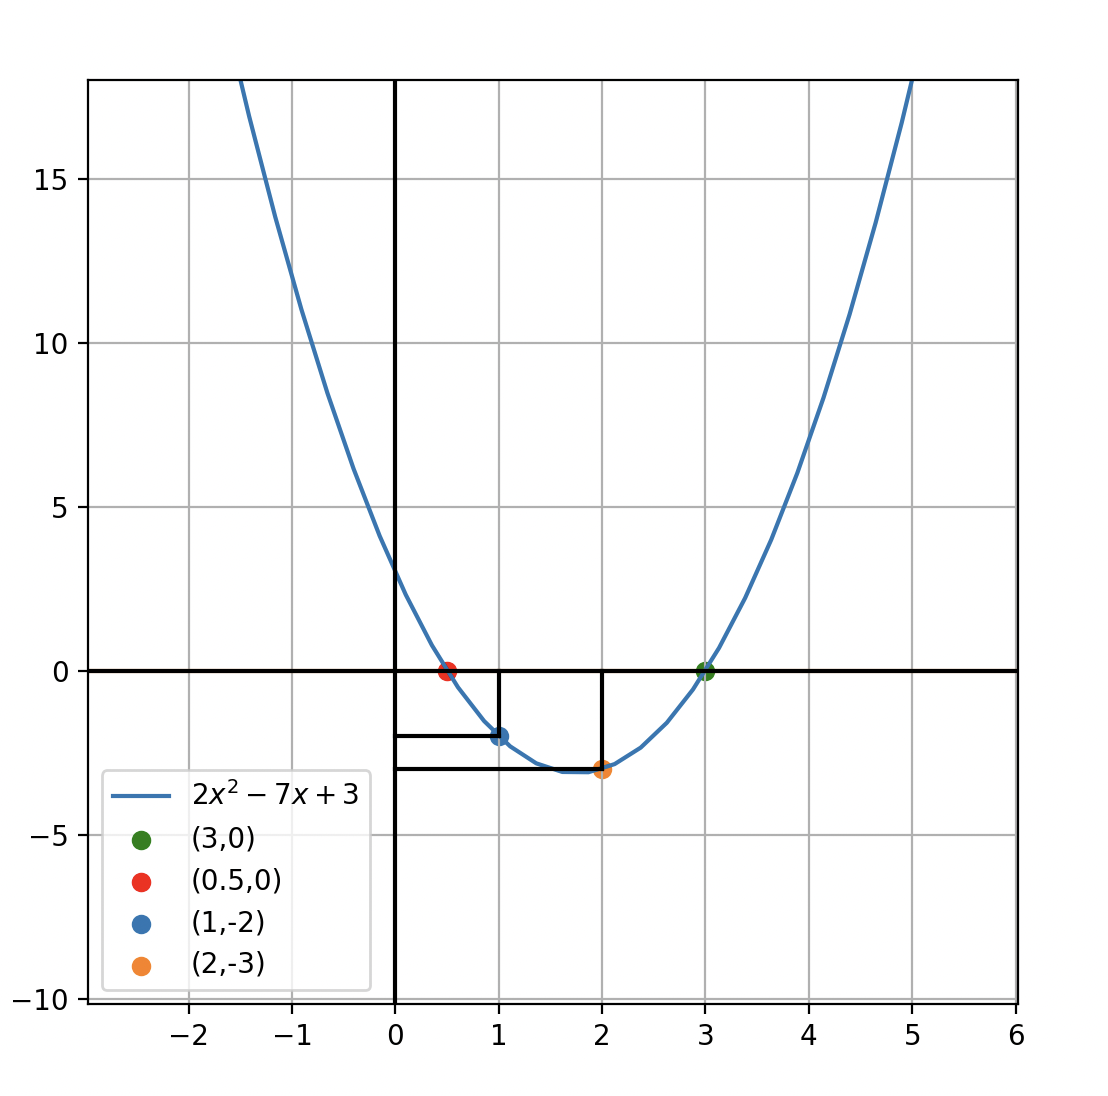
\includegraphics[width=0.6\columnwidth]{Figs/9416.png}
    \caption{Plot}
    \label{fig:placeholder}
\end{figure}
\end{frame}

\end{document}